\section{Futur de JavaScript}

\label{ch:futur}

Le futur de JavaScript est extrêmement lié au futur du web et plus généralement à l'évolution de l'informatique.

L'avenir du web est un sujet périlleux, car il est toujours difficile de cerner une tendance (l'année prochaine) et futurologie (dans 10ans).

Pour ce mémoire, je vais essayer de donner mon point de vue sur l'évolution d'internet et pourquoi j'ai décidé de parler de JavaScript et mise sur lui comme un acteur majeur de cette évolution. Comprenez par là que c'est mon avis et qu'a travers les parties que j'ai présenté dans mon mémoire vous êtes libres ou non d’adhérer à mon avis.

\subsection{Du web 1.0 au web 2 squarred}

JavaScript a actuellement 18ans et le moins que l'on puisse dire, c'est qu'en 18ans, tout à changé même si les fondements sont toujours là. De nouveaux usages se sont développé et se développent encore, mais ils se cumulent avec les anciens, du moins pour les technologies grand public. Depuis les années 2000 et la bulle d'internet, je ne pense pas me tromper en disant que l'histoire du web s'écrit par cycle de 5 ans marqué par la domination d'acteur sur-puissants. Les années 2000 ont été les années des portails (Yahoo, MSN, AOL...) qui concentraient l'audience avec une offre exhaustive de contenus et se services. Les années 2005 sont les années de Google et de son moteur de recherche concentrant plus de 80\% du marché. Les années 2010, dans lesquels nous nous trouvons, sont marquées par la domination des réseaux sociaux et notamment Facebook qui comporte quasiment 1 milliard d'utilisateurs.

Puisque nous évoquons l'histoire de l'évolution du web, il me parait indispensable de parler brièvement des grands stades d'évolution.

\begin{list}{•}{}

\item

Le web 1.0, centré sur les \textbf{documents}, avec la généralisation d'outils comme l'email, des portails de contenus ainsi que le commerce en ligne;

\item

Le web 2.0, centré sur les \textbf{utilisateurs}, avec la généralisation des réseaux sociaux, de contenus générés par les utilisateurs, les pratiques du social shopping et de nombreuses innovations autour des API et mashups;

\item

Le web squarred, centré sur les données, principalement axé sur la circulation temps-réel de l'information. Les données sont agrégées dans des écosystèmes, qui sont rattachés à tous types d’objets (ombres informationnelles) et générées de façon mécanique (métadonnées implicites) ;

\item

Le web 3.0, centré sur les agents intelligents, mais ceci n'est pour l'instant qu'un concept abstrait.

\end{list}

\begin{center}

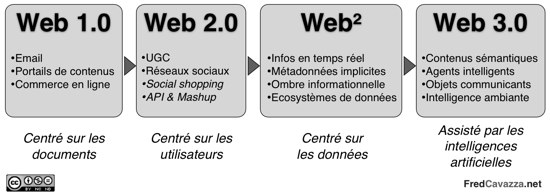
\includegraphics[scale=0.8]{img/Web1-3.jpg}

\label{Les grandes étapes d'évolutions du web}

\end{center}

\subsection{Pourquoi parler du Web Squared ?}

Je suis persuadé que nous sommes à la fin du web 2.0, l'émergence des terminaux mobiles a bousculé le marché et a ouvert la prochaine grosse itération du web: le web en temps réel, la réalité augmenté, les objets communicants, le cloud sont des innovations en cours de maturation qui vont entièrement changer notre façon de consommer, travailler et communiquer.

\subsection{L'essor du temps réel: un cerveau collectif}

Le microblogging est la révolution qui oblige l'informatique à devenir temps réel. Alors que le blogging a ajouté des dizaines de millions de sites à indexer chaque jour et même chaque heure, le microblogging nécessite une mise à jour instantanée. Cette nécessité implique de profond changement à la fois dans l'infrastructure et dans la méthode. La recherche d'un sujet populaire sur Twitter par exemple est confronté au message suivant "Voyez ce qu'il se passe maintenant" suivi, quelques instant plus tard par "42 résultats supplémentaires. Actualisez la page pour les consulter."

La recherche en temps réel encourage la réponse en temps réel. Twitter étant massivement temps réel est devenus en peu de temps, la première source d'informations dans le monde. Avec des services comme les mises à jour de statut des réseaux sociaux, une nouvelle source de données a été ajoutée au Web. Des modifications en temps réel et qui sont devenu indispensable pour la plupart d'entre nous.

L'utilisation du temps réel notamment par Twitter à provoqué de profond changement dans notre société, tant au niveau économique, politique que sociétale.

Le Guatemala et l'Iran ont tous deux ressenti l'effet Twitter, les protestations politiques ayant été lancées et coordonnées sur Twitter.

\subsection{Et JavaScript dans tout ça?}

JavaScript est par nature un langage événementiel ce qui le rend parfait pour les applications nécessitant le temps réel. Comme je viens de l'expliquer récemment, le temps réel est la prochaine évolution du Web. Le web squarred annonce d'après moi la révolution de JavaScript dans l'informatique et le juste retour du bâtons. Grâce à l'émergence du temps réel, JavaScript va enfin prouver ce dont il est capable. Node.js et Socket.IO en sont les exemple vivant de toute ce bouillonnement autour de lère du temps réel. JavaScript est tellement préparé au temps réel que tout les frameworks cotés clients l'ont prévue. Le nouveaux standard de EcmaScript (Harmony) et CommonJS prépare JavaScript à devenir un acteur de choix dans le développement d'application à but temps réel.



